\SourcePage{367}{370}
\section{Crossing of electronic terms}

The electronic terms of a diatomic molecule, regarded as functions of the internuclear distance $r$, may be displayed graphically by plotting the energy against $r$. Whether curves representing different terms can cross is an important question.

Let $U_1(r)$ and $U_2(r)$ be two different electronic terms. If they intersect at some point, then near that point their values are close. It is convenient to formulate the question of whether such an intersection is possible as follows.

Consider a point $r_0$ at which $U_1(r)$ and $U_2(r)$ have very close but unequal values, denoted by $E_1$ and $E_2$, and ask whether the two terms can be made equal by shifting the point through a small amount $\delta r$. The energies $E_1$ and $E_2$ are eigenvalues of the Hamiltonian $\widehat H_0$ for the electrons in the field of nuclei separated by $r_0$. If $r$ is increased by $\delta r$, the Hamiltonian becomes $\widehat H_0+\widehat V$, where $\widehat V=\delta r\,\partial\widehat H_0/\partial r$ is a small correction. The values of $U_1$ and $U_2$ at $r_0+\delta r$ may be treated as eigenvalues of this new Hamiltonian. Thus perturbation theory can be used to determine the two terms at $r_0+\delta r$, with $\widehat V$ regarded as a perturbation of $\widehat H_0$.

The ordinary perturbation method is not applicable here, since the unperturbed eigenvalues $E_1$ and $E_2$ lie very close together and their difference need not be large compared with the perturbation; condition (38.9) is not satisfied. As $E_2-E_1\to0$ the eigenvalues become degenerate, so for neighboring eigenvalues it is natural to use a method analogous to that developed in \S~39.

Let $\psi_1$ and $\psi_2$ be eigenfunctions of the unperturbed operator $\widehat H_0$ belonging to $E_1$ and $E_2$. Instead of $\psi_1$ and $\psi_2$ themselves, take as the initial zeroth approximation their linear combinations
\begin{equation}
 \psi=c_1\psi_1+c_2\psi_2.
 \tag{79.1}
\end{equation}

\SourcePage{368}{371}
Substitution in the perturbed equation
\begin{equation}
 (\widehat H_0+\widehat V)\psi=E\psi
 \tag{79.2}
\end{equation}
gives
\[
 c_1(E_1+\widehat V-E)\psi_1+c_2(E_2+\widehat V-E)\psi_2=0.
\]
Multiplying this equation on the left in turn by $\psi_1^*$ and $\psi_2^*$ and integrating, we obtain two algebraic equations:
\begin{equation}
 \left.\begin{aligned}
 c_1(E_1+V_{11}-E)+c_2V_{12}&=0,\\
 c_1V_{21}+c_2(E_2+V_{22}-E)&=0.
 \end{aligned}\right\}
 \tag{79.3}
\end{equation}
Because $\widehat V$ is Hermitian, $V_{11}$ and $V_{22}$ are real and $V_{12}=V_{21}^*$. The compatibility condition is
\[
 \begin{vmatrix}E_1+V_{11}-E&V_{12}\\V_{21}&E_2+V_{22}-E\end{vmatrix}=0,
\]
and hence
\begin{equation}
 E=\frac12(E_1+E_2+V_{11}+V_{22})\pm
 \sqrt{\frac14(E_1-E_2+V_{11}-V_{22})^2+|V_{12}|^2}.
 \tag{79.4}
\end{equation}
This formula gives the required energy eigenvalues to first approximation.

If the energies of the two terms become equal at $r_0+\delta r$, the two values of $E$ in (79.4) must coincide. The expression under the radical must therefore vanish. Since it is a sum of two squares, the conditions for a crossing are
\begin{equation}
 E_1-E_2+V_{11}-V_{22}=0,\qquad V_{12}=0.
 \tag{79.5}
\end{equation}
But there is only one arbitrary parameter specifying the perturbation $\widehat V$, namely the displacement $\delta r$. Consequently the two equations (79.5) cannot in general be satisfied simultaneously (we suppose that $\psi_1$ and $\psi_2$ have been chosen real, so that $V_{12}$ is real as well).

It may happen, however, that $V_{12}$ vanishes identically. Only one

\SourcePage{369}{372}
equation (79.5) then remains, and it can be satisfied by a suitable choice of $\delta r$. This occurs whenever the two terms have different symmetry. Here symmetry includes every possible kind: symmetry under rotations about the axis, reflections in planes, inversion, and permutations of electrons. For a diatomic molecule, the two terms may differ in $\Lambda$, parity, or multiplicity; two $\Sigma$ terms may also differ as $\Sigma^+$ and $\Sigma^-$.

This statement follows because the perturbation operator, like the Hamiltonian itself, commutes with all the molecular symmetry operators: the angular-momentum operator about the axis, the reflection and inversion operators, and the electron-permutation operators. It was shown in \S\S~29 and 30 that a scalar quantity whose operator commutes with the angular-momentum and inversion operators can have nonzero matrix elements only between states of equal angular momentum and parity. Essentially the same proof applies to an arbitrary symmetry operator. We shall not repeat it here, particularly since \S~97 will give another general proof based on group theory.

We thus reach the conclusion that, in a diatomic molecule, only terms of different symmetry can cross; terms of the same symmetry cannot cross (E.~Wigner, J.~von Neumann, 1929). If an approximate calculation produced two crossing terms of the same symmetry, the next approximation would separate them, as shown by the solid curves in Fig.~27.

This result is not restricted to diatomic molecules. It is in fact a general theorem of quantum mechanics, valid whenever the Hamiltonian contains a parameter and its eigenvalues are consequently functions of that parameter.

In group-theoretical language (see \S~96), the general requirement for terms to cross is that they belong to different irreducible representations of the symmetry group of the system's Hamiltonian\footnote{The electronic terms of the $\mathrm H_2^+$ ion appear to be an exception. They are characterized by the angular-momentum projection $\Lambda$ and two elliptic quantum numbers $n_\xi,n_\eta$ (see the problem in \S~78). Since these numbers belong to functions of different variables, there is in general no reason to prevent the crossing of terms $E(R)$ that have the same $\Lambda$ but different pairs $n_\xi,n_\eta$, although such terms have the same symmetry under rotations and reflections. In fact, however, separability of the variables in the Schrödinger equation means that the Hamiltonian has a higher symmetry than its geometric properties alone imply; with respect to this full symmetry group, states of different $n_\xi,n_\eta$ belong to different types.}.

\SourcePage{370}{373}
For a polyatomic molecule, the electronic terms depend not on one parameter but on several---the distances between the various nuclei.

Let $s$ be the number of independent internuclear distances; for an $N$-atom molecule ($N>2$) with an arbitrary nuclear configuration, $s=3N-6$. Geometrically, every term $U_n(r_1,\ldots,r_s)$ is a surface in a space of $s+1$ dimensions. Intersections of these surfaces may occur along manifolds whose dimensionality ranges from 0 (an isolated point) to $s-1$.

\begin{figure}[ht]
\centering
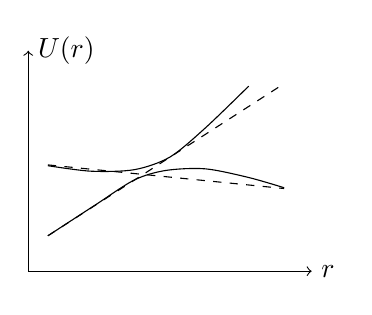
\begin{tikzpicture}[x=1cm,y=1cm]
 \draw[->] (0,0)--(3.6,0) node[right] {$r$};
 \draw[->] (0,0)--(0,2.8) node[right] {$U(r)$};
 \draw[dashed] (.25,.45)--(3.2,2.35);
 \draw[dashed] (.25,1.35)--(3.25,1.05);
 \draw[smooth] plot coordinates {(.25,1.34)(.8,1.27)(1.35,1.29)(1.8,1.45)(2.25,1.82)(2.8,2.35)};
 \draw[smooth] plot coordinates {(.25,.45)(.85,.84)(1.35,1.16)(1.75,1.28)(2.25,1.30)(2.8,1.19)(3.25,1.06)};
\end{tikzpicture}
\caption*{Fig. 27}
\end{figure}

The foregoing argument remains fully valid, except that the perturbation $\widehat V$ is now specified not by one parameter but by $s$ of them, the displacements $\delta r_1,\ldots,\delta r_s$. With as few as two parameters, however, the two equations (79.5) can in general be satisfied. Thus, in polyatomic molecules any pair of terms can cross. If the terms have the same symmetry, their crossing is fixed by the two conditions (79.5), and the intersection manifold has dimension $s-2$. For terms of different symmetry only one condition remains, and the intersection manifold has dimension $s-1$.

For example, when $s=2$, the terms are surfaces in a three-dimensional coordinate system. If the terms have different symmetry, these surfaces intersect along lines ($s-1=1$); if their symmetry is the same, they intersect at points ($s-2=0$). The form of the surfaces near such an isolated intersection is easily found. The energies near a crossing point are given by (79.4). In that expression the matrix elements $V_{11}$, $V_{22}$, and $V_{12}$ are linear functions of $\delta r_1$, $\delta r_2$, and hence linear

\begin{figure}[ht]
\centering
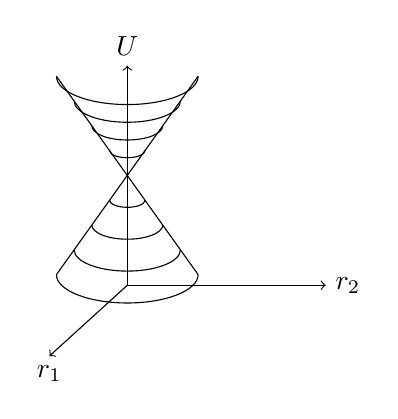
\begin{tikzpicture}[x=.9cm,y=.9cm]
 \draw[->] (0,0)--(0,3.1) node[above] {$U$};
 \draw[->] (0,0)--(2.8,0) node[right] {$r_2$};
 \draw[->] (0,0)--(-1.1,-1.0) node[below] {$r_1$};
 \foreach \h/\rx/\ry in {.35/.25/.10,.7/.5/.2,1.05/.75/.3,1.4/1/.4}
   {\draw (-\rx,1.55+\h) arc[start angle=180,end angle=360,x radius=\rx,y radius=\ry];
    \draw (-\rx,1.55-\h) arc[start angle=180,end angle=360,x radius=\rx,y radius=\ry];}
 \draw (-1,2.95)--(0,1.55)--(1,2.95);
 \draw (-1,.15)--(0,1.55)--(1,.15);
\end{tikzpicture}
\caption*{Fig. 28}
\end{figure}

\SourcePage{371}{374}
functions of the distances $r_1$, $r_2$ themselves. As is known from analytic geometry, such an equation describes an elliptic cone. Near a crossing point, therefore, the terms form a two-napped elliptic cone of arbitrary orientation (Fig.~28).
